%
% wegintegral.tex -- Wegintegral
%
% (c) 2025 Prof Dr Andreas Müller, OST Ostschweizer Fachhochschule
%
\bgroup
\definecolor{darkred}{rgb}{0.8,0,0}
\definecolor{darkgreen}{rgb}{0,0.6,0}
\begin{frame}[t]
\setlength{\abovedisplayskip}{5pt}
\setlength{\belowdisplayskip}{5pt}
\frametitle{Wegintegral einer 1-Form}
\vspace{-20pt}
\begin{columns}[t,onlytextwidth]
\begin{column}{0.52\textwidth}
\begin{definition}[Wegintegral]
Für den Weg \(\gamma\colon[t_A,t_B]\to\mathbb{R}^n:t\mapsto \gamma(t)\) und
eine 1-Form $\alpha$ ist
\[
\int_\gamma
\alpha
=
\int_{t_A}^{t_B}
\langle \alpha(\gamma(t)),\dot{\gamma}(t)\rangle\,dt
\]
\end{definition}
\uncover<2->{%
\begin{block}{Hauptsatz}
\[
\int_\gamma {\color{darkgreen}df}
\uncover<3->{=
\int_A^B {\color{darkgreen}df}}
\uncover<4->{=
\int_\gamma \sum_{i=1}^n \frac{\partial f}{\partial x^i}\,dx^i}
\uncover<5->{=
f(A) - f(B)}
\]
\end{block}}
\uncover<6->{%
\begin{block}{Wegunabhängigkeit?}
Unter welchen Voraussetzungen ist
\[
\int_{\gamma_1} \alpha
=
\int_{\gamma_2} \alpha
\,\text{?}
\]
\end{block}}
\end{column}
\begin{column}{0.44\textwidth}
\begin{center}
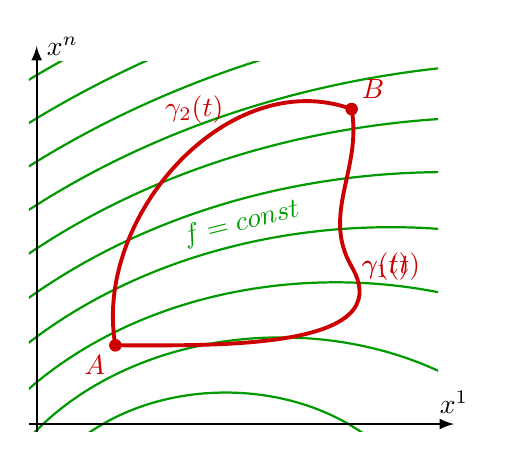
\begin{tikzpicture}[>=latex,thick]
\begin{scope}
	\clip (-0.1,-0.1) rectangle (5.1,4.6);
	\uncover<2->{
	\foreach \r in {1,...,12}{
		\draw[color=darkgreen] ({1+0.7*\r},{-1-0.3*\r})
			ellipse({1.3*\r} and {1.0*\r});
	}
	\node[color=darkgreen] at (2.6,2.55) [rotate=14] {$f=\text{const}$};
	}
\end{scope}
\coordinate (A) at (1,1);
\coordinate (B) at (4,4);
\coordinate (C) at (4,2);
\draw[line width=1.4pt,color=darkred]
	(A) to[out=0,in=-60]
	(C) to[out=120,in=-80] (B);
\uncover<6->{
\draw[line width=1.4pt,color=darkred]
	(A) to[out=100,in=160] (B);
}
\draw[->] (-0.1,0) -- (5.3,0) coordinate[label={$x^1$}];
\draw[->] (0,-0.1) -- (0,4.8) coordinate[label={right:$x^n$}];
\fill[color=darkred] (A) circle[radius=0.08];
\fill[color=darkred] (B) circle[radius=0.08];
\node[color=darkred] at (A) [below left] {$A$};
\node[color=darkred] at (B) [above right] {$B$};
\uncover<1-5>{
\node[color=darkred] at (C) [right] {$\gamma(t)$};
}
\uncover<6->{
\node[color=darkred] at (C) [right] {$\gamma_1(t)$};
\node[color=darkred] at (2,4) {$\gamma_2(t)$};
}
\end{tikzpicture}
\end{center}
\end{column}
\end{columns}
\end{frame}
\egroup
